    \documentclass[12pt,letter]{article}
    \usepackage[utf8]{inputenc}
    \usepackage{fontspec}
    \usepackage{xltxtra}
    \setmainfont{Comfortaa}
    \usepackage{amsmath}
    \usepackage{amsfonts}
    \usepackage{amssymb}
    \usepackage{float}
    \usepackage{makeidx}
    \usepackage{graphicx}
    \usepackage{listings}
    \usepackage{color}
    \usepackage[none]{hyphenat}
    \usepackage{fancyhdr}
    \usepackage{titlesec}
    \usepackage{imakeidx}
    \usepackage{lscape}
    \usepackage{makeidx}
    \usepackage{graphicx}
    \usepackage{color}
    \usepackage{colortbl}
    \usepackage{booktabs}
    \usepackage{setspace} 
    \usepackage{rotating} 
    \usepackage{hyperref}
     \usepackage[final]{pdfpages}
    \usepackage[babel]{csquotes}
    \usepackage[spanish]{babel}
    \usepackage[style=apa]{biblatex}
    \hypersetup{
    colorlinks=true, %set true if you want colored links
    linktoc=all,     %set to all if you want both sections and subsections linked
    linkcolor=blue,  %choose some color if you want links to stand out
    linktocpage,
    colorlinks,}
	\definecolor{gray97}{gray}{.97}
	\definecolor{gray75}{gray}{.75}
	\definecolor{gray45}{gray}{.45}
	\usepackage{booktabs}
	\usepackage{setspace} 
	\usepackage{rotating} 
	\usepackage{listings}
	\usepackage{textcomp}
	\lstset{
	language=python,
	framerule=0pt,
	aboveskip=0.5cm,
	framextopmargin=3pt,
	framexbottommargin=3pt,
	framexleftmargin=0.4cm,
	framesep=0pt,
	rulesep=.4pt,
	backgroundcolor=\color{gray97},
	rulesepcolor=\color{black},
	%
	stringstyle=\ttfamily,
	showstringspaces = false,
	basicstyle=\small\ttfamily,
	commentstyle=\color{gray45},
	keywordstyle=\bfseries,
	%
	numbers=left,
	numbersep=15pt,
	numberstyle=\tiny,
	numberfirstline = false,
	breaklines=true,
		}

    \usepackage[ocgcolorlinks]{ocgx2}
    \usepackage[final]{pdfpages}
    \usepackage[left=3cm, right=2.4cm, top=2.5cm, bottom=2.7cm]{geometry}%aqui estamos poniendo los limites
    \renewcommand{\baselinestretch}{1.5}%esto es el interlineado 1.5 para nuestros textos
    \renewcommand{\contentsname}{ÍNDICE GENERAL}%esto es para modificar el nombre del indice de contenidos
    \renewcommand{\listfigurename}{ÍNDICE DE FIGURAS}%esto es para modificar el nombre del indice de figuras
    \renewcommand{\listtablename}{ÍNDICE DE TABLAS}%esto es para modificar el nombre del indice de tablas
    \renewcommand{\figurename}{{\bf FIGURA}}%con esto modificamos los nombres de las figuras en la leyenda
    \renewcommand{\tablename}{{\bf TABLA}}%con esto modificamos los nombres de las tablas en la leyenda
%    \renewcommand{\chaptername}{CAPÍTULO}
    \renewcommand{\indexname}{ÍNDICE ALFABÉTICO}
    \makeindex
    
\begin{document}
\sloppy 

	\thispagestyle{empty}
	\begin{center}
		{\fontsize{20}{40}\selectfont UNIVERSIDAD MAYOR DE SAN ANDRES}\\
		\vspace*{0.2cm}
		{\fontsize{16}{32}\selectfont FACULTAD DE CIENCIAS PURAS Y NATURALES}\\
		{\fontsize{14}{28}\selectfont {\it CARRERA DE INFORMÁTICA}}\\
	\end{center}
	\begin{figure}[h]
	\centering
	
\includegraphics[width=0.20\linewidth]{im/LOGO}
	\end{figure}
	\begin{center}
		
		
	{\textcolor{red}{\fontsize{24}{0}\selectfont Examen Parcial - Pregunta 3}}\\
	\end{center}
	\hspace*{0.1cm}
	\begin{center}
		\begin{tabular}{r l l}
			\toprule
			{\fontsize{16}{38}\selectfont {\bf Nombres:}} & {\fontsize{14}{38}\selectfont  EDUARDO MEDRANO AYARDE }&CI: 6989411 \\
			 
			
		 
		 
		 \toprule
		 %{\fontsize{16}{38}\selectfont {\bf CI:}} & {\fontsize{14}{38}\selectfont 6989411}\\

			 
		 \toprule
			{\fontsize{16}{38}\selectfont {\bf Materia:}} & {\fontsize{14}{38}\selectfont Inteligencia Artificial (INF-354)}\\
			\toprule
			{\fontsize{16}{38}\selectfont {\bf Docente:}} & {\fontsize{14}{38}\selectfont M.Sc. Moises Martin Silva Choque}\\
			\toprule
			{\fontsize{16}{38}\selectfont {\bf Fecha:}} & {\fontsize{14}{38}\selectfont \today}\\
			\bottomrule
		\end{tabular}
	
	\end{center}
		
	
	 
	
	
	
	

%a partir de aca vamos a ejecutar tipo de indice romano 
\pagenumbering{Roman}%mayuscula y vamos a resetear el indice apartir de aca
\setcounter{page}{1}%ahora podemos continuar con el formato establecido


\newpage
\setcounter{page}{2}



\pagenumbering{arabic}


\setcounter{section}{0}
\newpage



\section{\fontsize{14}{0}\selectfont Use 3 columnas del dataset, generándose un algoritmo genético con el uso de DEAP}
\subsection{ Descripción del Dataset}
Para el caso de estudio con el DEAP, se hizo uso del dataset Haberman, del siguiente enlace \url{https://archive.ics.uci.edu/ml/datasets/Haberman\%27s+Survival}, el cual describe, sobre la evolución y supervivencia de mujeres que hayan sido operadas, para tratar el cáncer de mama, las columnas del dataset son los siguientes: 
\begin{itemize}
	\item Edad: Edad de las mujeres, cuando fueron sometidas a la operación. 
	\item Año de intervención quirúrgica: restando 2000-1900, la columna muestra el año en el que se realizaron la operación. 
	\item Ganglios: Es un número entero, que nos señala, cuantos ganglios cancerosos fueron detectados.
	\item Supervivencia: 1 si sobrevivió más de 5 años después de la operación, 2 si murió entre los 5 años.  
\end{itemize}
Para el uso del DEAP, se hara uso de las 3 primeras columnas.\\
El proceso de evolución genética, nos dirá cuantas generaciones se necesitaran, para que mujeres de 21 años ya presenten cáncer de mama. Para este propósito el algoritmo se desarrolla bajo las siguientes características:
\begin{itemize}
	\item Se evaluaran grupos de 10 mujeres en 10 mujeres.
	\item La población será de 1000 mujeres.
	\item Será una función de minimización, esto por el hecho de que se desea ver a mujeres jóvenes y cuantas generaciones se tomara.
	\item En la función de evaluación se tiene los siguientes parámetros:
	\begin{itemize}
		\item Se hará una sumatoria de todos los ganglios cancerosos encontrados en el grupo de 10 mujeres.
		\item La sumatoria se realiza solo si, el grupo de estudio se encuentra en el rango de edad del dataset, el año de la cirugía fue entre 1960-1970 y por último la edad de la mujer fue menor a 35 años. 
		\item Al cumplir esto se pregunta si la sumatoria de ganglios cancerosos, es mayor a 10, de ser así se devuelve el valor máximo del grupo de estudio, caso contrario se devuelve a la más joven.
		
	\end{itemize}
	\item El algoritmo de cruce es cxUniform.
	\item La población es aleatoria en un rango de edad de 21 a 80 años.
	
\end{itemize}
Todo el análisis anterior, está desarrollado bajo el siguiente código:

\begin{lstlisting}[language=python]
import array
import random
import numpy
import pandas as pd
from deap import algorithms
from deap import base
from deap import creator
from deap import tools

#leemos los datos provenientes del dataset

data=pd.read_csv("haberman.csv",sep=",")
creator.create("FitnessMax", base.Fitness, weights=(-1.0,))
creator.create("Individual", list, fitness=creator.FitnessMax)
toolbox = base.Toolbox()

#colocamos en el grupo de mujeres que se someten a una operación por cancer de mama entre 21 y 50 años
toolbox.register("attr_bool", random.randint, 21, 80)
toolbox.register("individual", tools.initRepeat, creator.Individual, toolbox.attr_bool, 10)
toolbox.register("population", tools.initRepeat, list, toolbox.individual)

def evacancer(individual,edad,t_opera,ganglios_auxiliares):

#vemos cuantas mujeres sometidas a operación generaron ganglios cancerosos en el grupo de 10 mujeres
	aux=0
	gnp=numpy.array(ganglios_auxiliares)
	enp=numpy.array(edad)
	indi=numpy.array(individual)
	for a in range(0,len(individual)-1):
		if individual[a] in edad and t_opera[a]>60 and edad[a]<35:
		aux+=gnp[a]
#ya definido los ganglios generados entre todas las mujeres podemos decir que si 
# sumados todos los ganglios cancerosos el numero es mayo o igual que 10 
# el conjunto de mujeres que no estaba en el rango de edad para generar ganglios cancerosos, generara 1 
# caso contrario no generara ningun ganglio
# y en un caso devolvemos la mujer de mas edad o la mas joven 
if aux>=10:
	return indi.max(),
else:
	return indi.min(),
toolbox.register("evaluate", evacancer,edad=data["edad"],t_opera=data["year"],ganglios_auxiliares=data["auxilia"])
toolbox.register("mate", tools.cxUniform, indpb=0.5)
toolbox.register("mutate", tools.mutFlipBit, indpb=0.05)
toolbox.register("select", tools.selTournament, tournsize=3)

def main():
	pop = toolbox.population(n=1000)
	hof = tools.HallOfFame(1)
	stats = tools.Statistics(lambda ind: ind.fitness.values)
	stats.register("avg", numpy.mean)
	stats.register("std", numpy.std)
	stats.register("min", numpy.min)
	stats.register("max", numpy.max)
	pop, log = algorithms.eaSimple(pop, toolbox, cxpb=0.5, mutpb=0.2, ngen=20, 
	stats=stats, halloffame=hof, verbose=True)
	return pop, log, hof
if __name__ == "__main__":
main()
\end{lstlisting}
De donde se obtiene los siguientes resultados:
\begin{figure}[H]
	\centering
	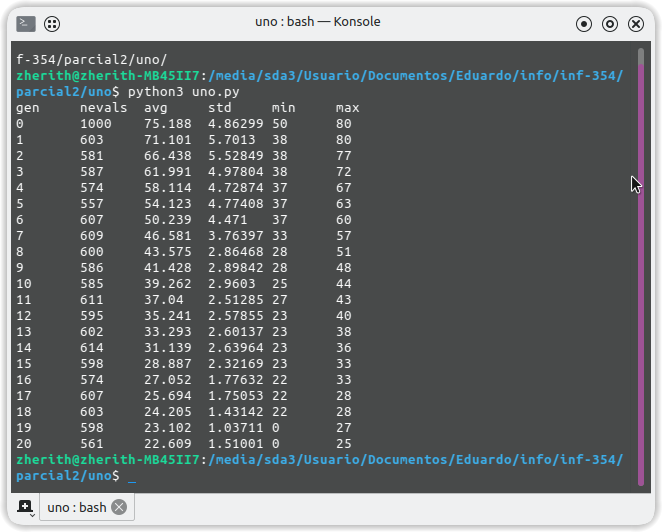
\includegraphics[width=0.8\linewidth]{im/uno.png}
	\caption[Resultados Obtenidos del Dataset Haberman]{Resultados Obtenidos del Dataset Haberman}
\end{figure}
De donde se puede apreciar que, para la generación 18, mujeres entre el rango de edad de 22 a 28, pueden presentar ganglios cancerosos.






%introduccion 
\newpage

\end{document}
